% Revisão consolidada: 25/11/2026. Não antecipa resultados finais.
\chapter{Arquitetura geral do DoseCerta}
\section{Visão sistêmica e distribuição de responsabilidades}
A configuração planejada compreende um módulo central, dois intermediários e oito submódulos, com quatro posições por intermediário. Cada submódulo armazena um medicamento. A central utiliza Raspberry Pi Zero 2 W; cada intermediário e submódulo utiliza ESP32. Isso corresponde a dez ESP32 previstas, sem implicar que todas tenham sido montadas e aceitas. \cite{DC_CIRCUITOS}
A Raspberry Pi coordena agenda, execução local, persistência, comunicação externa e periféricos centrais. O submódulo controla motor e leitura óptica; o intermediário identifica e sinaliza suas quatro posições e distribui fisicamente alimentação e barramento. A aplicação web e o agente não controlam diretamente as bobinas. \cite{DC_CIRCUITOS,DC_COMPILADO}
\section{Camadas e caminhos de informação}
O Care encaminha operações à API FastAPI, responsável pelas regras de cuidado e acesso aos dados centrais. A Raspberry Pi sincroniza com a API e mantém registros locais em SQLite. A conexão entre central e ESP32 utiliza o barramento compartilhado. O esquema do artigo ilustra a separação dessas camadas; detalhes de versões e de autenticação são tratados nos capítulos específicos. \cite{DC_APP,DC_ARTIGO}
\begin{figure}[htbp]\centering
\caption{Fluxo de autenticação e sincronização apresentado no artigo; esquema documental, não prova de integração da versão final.}
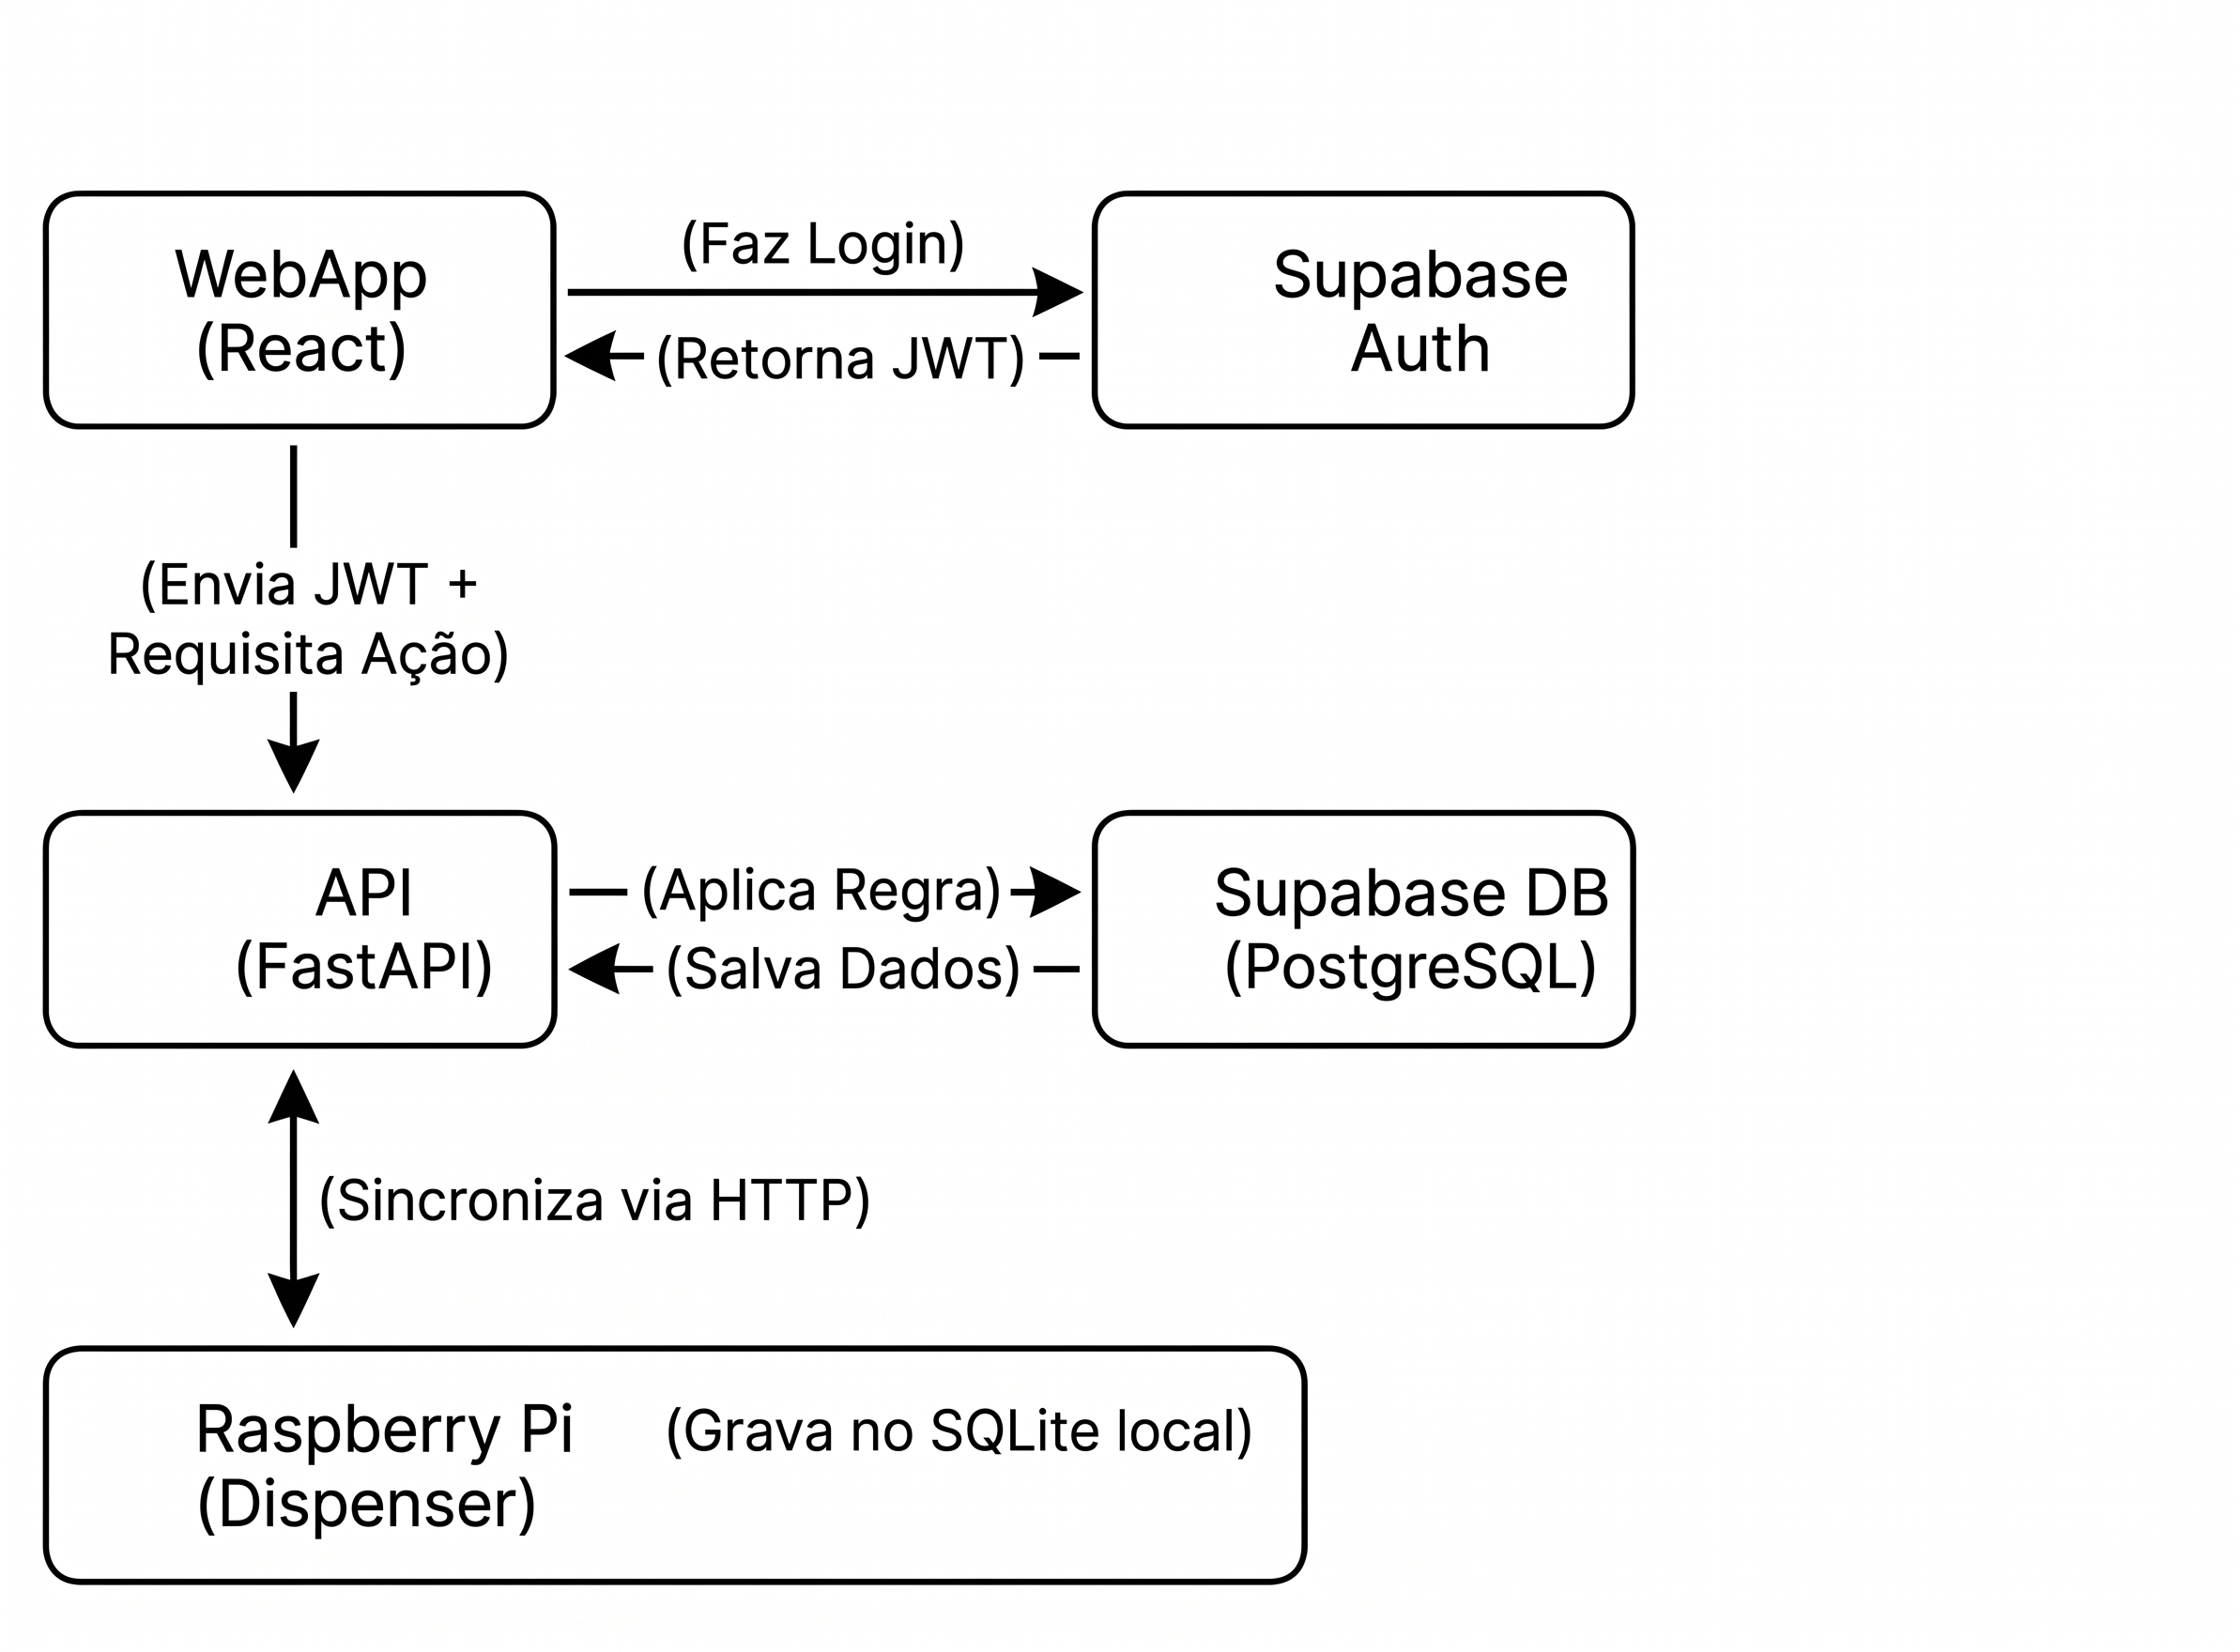
\includegraphics[width=0.82\textwidth,height=0.55\textheight,keepaspectratio]{Figuras/Artigo/arquitetura_artigo.png}
\fonte{Artigo e Anexo A, versão 2, material da equipe \cite{DC_ARTIGO}.}\end{figure}
\section{Arquitetura física e elétrica}
A ligação funcional possui quatro vias: +5 V, GND, SDA e SCL. Há um único SDA e um único SCL compartilhados; o intermediário os encaminha no mesmo nó aos submódulos e ao próximo andar, sem recriar outro barramento em GPIO diferentes. A Raspberry Pi é o controlador pretendido. A posição física dos contatos deve ser conferida por continuidade e não pela ordem de uma lista textual. \cite{DC_CIRCUITOS}
\section{Identidade, posição e conteúdo}
Endereço lógico, identidade de placa, posição física e medicamento são associações distintas. Mover um submódulo exige conferir e registrar a associação correspondente; um endereço não identifica automaticamente o conteúdo ou o novo local. O contrato posterior descreve instâncias e endereços derivados, mas a configuração realmente instalada deve ser comprovada por manifesto e leitura das placas. \cite{DC_COMPILADO}
\section{Evolução e divergências documentais}
O pré-relatório descreve Arduino Nano, conectores de cinco vias e fonte de 5 A; o mapa de setembro descreve ESP32, quatro vias e fonte prevista de 10 A. O artigo também preserva uma proposta de agente com Copilot Studio, enquanto a documentação de novembro relata Foundry e MCP. Esses registros pertencem a momentos e alcances diferentes; não são combinados em um circuito ou implantação supostamente únicos. \cite{DC_PREREL,DC_CIRCUITOS,DC_FOUNDRY}
\pendencia{ARQ01}{A autora enviará o subspace de arquitetura. Incorporar o diagrama da configuração final e confrontá-lo com esquema, versões e montagem real; não substituir o material prometido por inferência.}
\pendencia{ARQ02}{Fornecer esquema da montagem pós-reparos, orientação de cada pogo, continuidade e fotografias identificadas. O mapa funcional disponível não comprova ordem física nem estado atual de todos os módulos.}
\section{Estado relatado e restrições}
O registro de 12/11/2026 relata Raspberry Pi conectada, runtime 0.7.12, INT-01 0.3.1 e SUB-01 0.6.1 comunicando. Ao mesmo tempo informa ausência de RTC funcional, agenda automática desligada, \texttt{hardware\_ready=false} e necessidade de reconciliação do motor. Trata-se de uma fotografia documental datada, não de uma verificação executada nesta revisão nem de aceite final. \cite{DC_ANALISE}
\pendencia{ARQ04}{Confirmar a configuração na data de fechamento: hashes, versões, boot IDs, módulos montados, provisionamento e pré-condições de operação. Registrar RTC, agenda e comissionamento com evidências primárias.}
